\documentclass{beamer}
\mode<presentation>
{
  \usetheme{Warsaw}
}

\setbeamertemplate{navigation symbols}{}

%% For the formula
\usepackage{amsmath}
\usepackage{amsfonts}

\usepackage{pgfplots}

\usepackage{fancyvrb}
\usepackage{graphicx}
\usepackage{times}
\usepackage[T1]{fontenc}
\usepackage[english]{babel}
\usepackage[utf8]{inputenc}
\usepackage{color}
\usepackage[boxed]{algorithm}
\usepackage{algpseudocode}
%\usepackage{bchart}
\usepackage{amsmath}
\usepackage{amssymb}
\usepackage{float}
\usepackage{parcolumns}
\usepackage{listings}
\lstloadlanguages{
        erlang
}
\lstset{
  belowcaptionskip=1\baselineskip,
  breaklines=true,
  postbreak=\space\space, 
  breakindent=5pt,
  frameshape={RYRYNY}{y}{y}{RYRYNY},
  xleftmargin=\parindent,
  language=erlang,
  showstringspaces=false,
  basicstyle=\footnotesize\ttfamily,
  keywordstyle=\color{black},
  commentstyle=\itshape\color{gray!40!black},
  identifierstyle=\color{blue},
  stringstyle=\color{orange},
}

\title[ Lesser Evil]
{{\small Lesser Evil: \\ Embracing Failure to Protect Overall System Availability}
}
\author[Viktória Fördős, Alexandre Jorge Barbosa Rodrigues]
       {{\large
		Viktória Fördős, Alexandre Jorge Barbosa Rodrigues
       }}
\institute{
Cisco, Sweden
}
\date{{\scriptsize DAIS'22, Lucca}}

\begin{document}
\begin{frame}
  \titlepage
\end{frame}


\section{Motivation}
\subsection{Erlang Systems}
\begin{frame}{Erlang}
\begin{itemize}
\item Was designed in the Ericsson software technology lab for systems that will never stop or fail. 
\item First use case: multi-service switch, AXD 301.
\item A dynamically typed, concurrent, distributed, fault-tolerant, functional programming language. 
\item Is based on the actor model, an actor is an Erlang process.
\end{itemize}
\end{frame}

\begin{frame}{Erlang}
\begin{itemize}
\item Processes  can be started and stopped at any time.
\item Processes can fail.
\item Processes share nothing.
\item Processes are organised into applications. 
\item Multiple applications are deployed as one Erlang node. An Erlang node is one OS process.
\item Inspecting the processes and the runtime system have built-in support.
\end{itemize}
\end{frame}

\subsection{Embedded Systems}
\begin{frame}{Focus: Embedded Systems}
Embedded systems are widespread
\begin{itemize}
\item network elements,
\item military use cases,
\item IoT.
\end{itemize}

Embedded systems are expected to be responsive, and always available.

Embedded systems usually have
\begin{itemize}
\item weak processing capabilities,
\item very limited physical memory,
\item usually no virtual memory.
\end{itemize}

\end{frame}


\subsection{Embedded Device Controller}
\begin{frame}{Example use case: Embedded device controller}
\begin{itemize}
	\item The system is designed to run on and control an embedded device with limited memory and slow processing capability.
	\item The system and the device are expected to be always available.
%	\item The control system is written in Erlang.
\end{itemize}
\end{frame}

\begin{frame}{Normal operation}
\begin{itemize}
	\item The controller receives administrative requests that it processes, and as a result of processing, it executes commands on the embedded device. 
	\item The controller usually receives a few, small requests, but sometimes a large request arrives.
\end{itemize}
\end{frame}

\begin{frame}{Low memory conditions}
\begin{itemize}
	\item If a large request arrives when small requests are already being processed, the memory is not enough. 
	\item Device becomes unresponsive, worst case it even reboots.
	\item {\bfseries Does not satisfy high availability requirements.}
\end{itemize}
\end{frame}

\begin{frame}{Existing solutions}
The only solution to manage such situation is the Linux OOM Manager.
\begin{itemize}
	\item OOM Manager will terminate the controller.
	\item Device becomes unresponsive, worst case it even reboots.
	\item {\bfseries Does not satisfy high availability requirements.}
\end{itemize}
\end{frame}

\subsection{Problem Statement}
\begin{frame}{Problem Statement}
A more fine grained approach is needed, and is possible to give if the controller is implemented in Erlang.

\begin{itemize}
	\item The primary goal is to free up enough memory inside of the Erlang node to resume the normal operation of the controller.
	\item We accept local failures.
	\item We do not tolerate abnormal termination of the controller.
	\item Our goal is to prevent a major outage, but we accept temporary, partial system degradations.
\end{itemize}
\end{frame}

\section{Lesser Evil}
\begin{frame}{Our approach: Lesser Evil}
\begin{itemize}

\item Goal: Treat memory pressure of an Erlang system without the need of code modification. 

\item Idea: Monitor the running program and upon low memory conditions select some \emph{processes} with the greatest badness values and execute compensating actions on the selected processes. 
\end{itemize}
\end{frame}

%% Our approach is called Lesser Evil, the reason being that we prefer the Lesser Evil, which can be a system surving low memory conditions by allowing the system to operate on a potencially degraded state.

%% Our goal is to achieve this without the need for source code modification.

%% The idea phrase captures really well our approach, but in order to fully understand it we need to expand more on:
%% what processes are considered and why;
%% what is badness and how it's used
%% what are the compensating actions and how they are performed

\subsection{Entities}
\begin{frame}{Entities}
\begin{itemize}

\item Only a sub-set of the processes are considered, since some are critical.
\item The programmer instructs Lesser Evil on what processes should be considered, by selecting applications for Lesser Evil to monitor.

\end{itemize}
\end{frame}

\subsection{Badness}
\begin{frame}{Goal}
\begin{itemize}

\item Assign higher values to processes that have high memory usage and that will likely continue executing.
\item Assign lower values to processes that are long-lived, are important to the user and that several other processes depend on them (links, monitors).

\end{itemize}
\end{frame}

% Badness is the metric used to select which processes Lesser Evil should target. So Lesser Evil assigns...

\begin{frame}{Defining the badness metric}
$$
\mathit{badness} \equiv \frac{\mathit{Memory} * (\mathit{MessageQLength}+1)}{log_{10}(\mathit{Reds})*\mathit{Age}*(\mathit{Links}+1)*(\mathit{Mons}+1)*\mathit{Prio}}
$$

\begin{itemize}

\item MessageQLength - how much more tasks the process has pending.
\item Reds - amount of work the process has done.
\item Age - number of checks the process has survived.
\item Links and Mons - how central the process is.
\item Prio - process priority.

\end{itemize}

% Lesser evil calculates it based on the following formula

\end{frame}

% With regards to compensating actions, our in other words the evil part of Lesser Evil, the ones we selected are to trigger a full sweep GC on the Erlang process and terminating the Erlang process.
\subsection{Compensating actions}
\begin{frame}{Strategy}

Lesser Evil periodically collects metrics and activates itself on:
$$
\mathit{trigger}  \equiv \mathit{Mem} > 0.8 * \mathit{MemLimit}  \;\wedge \mathit{NotInCoolDownInterval}
$$

What compensating action is choosen:
$$
\mathit{select\_action}  \equiv \begin{cases}
    \mathit{trigger\_gc}       & \quad \text{if } \mathit{Mem} < \mathit{MemLimit} \\
    \mathit{terminate\_proc}  & \quad \text{otherwise}
  \end{cases}
$$

\end{frame}


%% The compensating actions are not harmless, triggering a full sweep garbage collection and terminating Erlang processes can influence negatively the normal functioning of the system, so lesser evil tries to lower the badness value for processes that are long-lived, are important to the user and that several other processes depend on them (links, monitors).


\section{Evaluation}
\subsection{Hyphotheses}
\begin{frame}{Hypotheses}
The goal of the evaluation is to confirm the following hypotheses.
\begin{itemize}

\item \emph{Hypothesis \#1: Lesser Evil can control the memory usage of an Erlang node, therefore, it helps an Erlang node survive low memory conditions.}
\item \emph{Hypothesis \#2: Lesser Evil can prevent major outages.}
\item \emph{Hypothesis \#3: Lesser Evil selects and executes actions on those processes that are mainly responsible for the memory usage and does not interfere with the rest of the processes.}
\item \emph{Hypothesis \#4: Lesser Evil's agent is non-intrusive to the Erlang node, its memory usage is low.}

\end{itemize}
\end{frame}

\subsection{Experiments}
\begin{frame}{Experiments}
\begin{itemize}
\item SUT: embedded device controller.
\item SUT runs in a Docker container: memory limit of 120 MB.
\item Load generation: 80\% small requests, 20\% large requests.
\item Linux OOM is active.
\item Two set of experiments: with and without Lesser Evil.
\end{itemize}
\end{frame}

\subsection{Results}
\begin{frame}{Results}
\begin{figure}[htbp]
\centering
\scalebox{.78}{
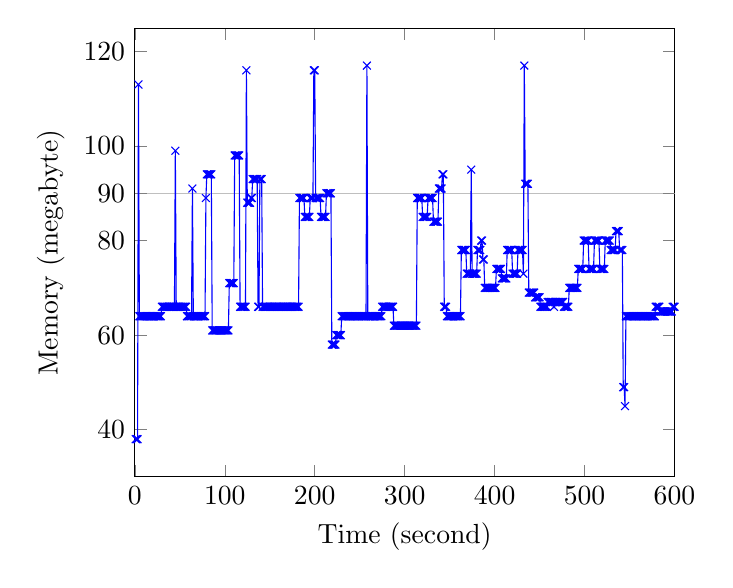
\begin{tikzpicture}
	\begin{axis}[
		xlabel=Time (second),
		xmin=0, xmax=600,
		extra y ticks={90},
		extra tick style={grid=major},
%		ymin=45000, ymax=160000,
%       scaled ticks=false,
%yticklabel style={
%        /pgf/number format/precision=0,
%        /pgf/number format/fixed
%},
		ylabel=Memory (megabyte),
%    legend style={
%        cells={anchor=east},
%        legend pos=outer north east,
%    }
]
	\addplot[color=blue,mark=x] coordinates {
(1   ,38)
(2   ,38)
(3   ,38)
(4   ,113)
(5   ,64)
(6   ,64)
(7   ,64)
(8   ,64)
(9   ,64)
(10  ,64)
(11  ,64)
(12  ,64)
(13  ,64)
(14  ,64)
(15  ,64)
(16  ,64)
(17  ,64)
(18  ,64)
(19  ,64)
(20  ,64)
(21  ,64)
(22  ,64)
(23  ,64)
(24  ,64)
(25  ,64)
(26  ,64)
(27  ,64)
(28  ,64)
(29  ,64)
(30  ,66)
(31  ,66)
(32  ,66)
(33  ,66)
(34  ,66)
(35  ,66)
(36  ,66)
(37  ,66)
(38  ,66)
(39  ,66)
(40  ,66)
(41  ,66)
(42  ,66)
(43  ,66)
(44  ,66)
(45  ,99)
(46  ,66)
(47  ,66)
(48  ,66)
(49  ,66)
(50  ,66)
(51  ,66)
(52  ,66)
(53  ,66)
(54  ,66)
(55  ,66)
(56  ,66)
(57  ,66)
(58  ,64)
(59  ,64)
(60  ,64)
(61  ,64)
(62  ,64)
(63  ,64)
(64  ,91)
(65  ,64)
(66  ,64)
(67  ,64)
(68  ,64)
(69  ,64)
(70  ,64)
(71  ,64)
(72  ,64)
(73  ,64)
(74  ,64)
(75  ,64)
(76  ,64)
(77  ,64)
(78  ,64)
(79  ,89)
(80  ,94)
(81  ,94)
(82  ,94)
(83  ,94)
(84  ,94)
(85  ,94)
(86  ,61)
(87  ,61)
(88  ,61)
(89  ,61)
(90  ,61)
(91  ,61)
(92  ,61)
(93  ,61)
(94  ,61)
(95  ,61)
(96  ,61)
(97  ,61)
(98  ,61)
(99  ,61)
(100 ,61)
(101 ,61)
(102 ,61)
(103 ,61)
(104 ,61)
(105 ,71)
(106 ,71)
(107 ,71)
(108 ,71)
(109 ,71)
(110 ,71)
(111 ,98)
(112 ,98)
(113 ,98)
(114 ,98)
(115 ,98)
(116 ,98)
(117 ,66)
(118 ,66)
(119 ,66)
(120 ,66)
(121 ,66)
(122 ,66)
(123 ,66)
(124 ,116)
(125 ,88)
(126 ,88)
(127 ,88)
(128 ,88)
(129 ,89)
(130 ,89)
(131 ,93)
(132 ,93)
(133 ,93)
(134 ,93)
(135 ,93)
(136 ,93)
(137 ,66)
(138 ,66)
(139 ,93)
(140 ,93)
(141 ,93)
(142 ,66)
(143 ,66)
(144 ,66)
(145 ,66)
(146 ,66)
(147 ,66)
(148 ,66)
(149 ,66)
(150 ,66)
(151 ,66)
(152 ,66)
(153 ,66)
(154 ,66)
(155 ,66)
(156 ,66)
(157 ,66)
(158 ,66)
(159 ,66)
(160 ,66)
(161 ,66)
(162 ,66)
(163 ,66)
(164 ,66)
(165 ,66)
(166 ,66)
(167 ,66)
(168 ,66)
(169 ,66)
(170 ,66)
(171 ,66)
(172 ,66)
(173 ,66)
(174 ,66)
(175 ,66)
(176 ,66)
(177 ,66)
(178 ,66)
(179 ,66)
(180 ,66)
(181 ,66)
(182 ,66)
(183 ,89)
(184 ,89)
(185 ,89)
(186 ,89)
(187 ,89)
(188 ,89)
(189 ,85)
(190 ,85)
(191 ,85)
(192 ,85)
(193 ,85)
(194 ,85)
(195 ,89)
(196 ,89)
(197 ,89)
(198 ,89)
(199 ,116)
(200 ,116)
(201 ,89)
(202 ,89)
(203 ,89)
(204 ,89)
(205 ,89)
(206 ,89)
(207 ,85)
(208 ,85)
(209 ,85)
(210 ,85)
(211 ,85)
(212 ,85)
(213 ,90)
(214 ,90)
(215 ,90)
(216 ,90)
(217 ,90)
(218 ,90)
(219 ,58)
(220 ,58)
(221 ,58)
(222 ,58)
(223 ,58)
(224 ,60)
(225 ,60)
(226 ,60)
(227 ,60)
(228 ,60)
(229 ,60)
(230 ,64)
(231 ,64)
(232 ,64)
(233 ,64)
(234 ,64)
(235 ,64)
(236 ,64)
(237 ,64)
(238 ,64)
(239 ,64)
(240 ,64)
(241 ,64)
(242 ,64)
(243 ,64)
(244 ,64)
(245 ,64)
(246 ,64)
(247 ,64)
(248 ,64)
(249 ,64)
(250 ,64)
(251 ,64)
(252 ,64)
(253 ,64)
(254 ,64)
(255 ,64)
(256 ,64)
(257 ,64)
(258 ,117)
(259 ,64)
(260 ,64)
(261 ,64)
(262 ,64)
(263 ,64)
(264 ,64)
(265 ,64)
(266 ,64)
(267 ,64)
(268 ,64)
(269 ,64)
(270 ,64)
(271 ,64)
(272 ,64)
(273 ,64)
(274 ,64)
(275 ,66)
(276 ,66)
(277 ,66)
(278 ,66)
(279 ,66)
(280 ,66)
(281 ,66)
(282 ,66)
(283 ,66)
(284 ,66)
(285 ,66)
(286 ,66)
(287 ,66)
(288 ,62)
(289 ,62)
(290 ,62)
(291 ,62)
(292 ,62)
(293 ,62)
(294 ,62)
(295 ,62)
(296 ,62)
(297 ,62)
(298 ,62)
(299 ,62)
(300 ,62)
(301 ,62)
(302 ,62)
(303 ,62)
(304 ,62)
(305 ,62)
(306 ,62)
(307 ,62)
(308 ,62)
(309 ,62)
(310 ,62)
(311 ,62)
(312 ,62)
(313 ,62)
(314 ,89)
(315 ,89)
(316 ,89)
(317 ,89)
(318 ,89)
(319 ,89)
(320 ,85)
(321 ,85)
(322 ,85)
(323 ,85)
(324 ,85)
(325 ,85)
(326 ,89)
(327 ,89)
(328 ,89)
(329 ,89)
(330 ,89)
(331 ,89)
(332 ,84)
(333 ,84)
(334 ,84)
(335 ,84)
(336 ,84)
(337 ,84)
(338 ,91)
(339 ,91)
(340 ,91)
(341 ,91)
(342 ,94)
(343 ,94)
(344 ,66)
(345 ,66)
(346 ,66)
(347 ,64)
(348 ,64)
(349 ,64)
(350 ,64)
(351 ,64)
(352 ,64)
(353 ,64)
(354 ,64)
(355 ,64)
(356 ,64)
(357 ,64)
(358 ,64)
(359 ,64)
(360 ,64)
(361 ,64)
(362 ,64)
(363 ,78)
(364 ,78)
(365 ,78)
(366 ,78)
(367 ,78)
(368 ,78)
(369 ,73)
(370 ,73)
(371 ,73)
(372 ,73)
(373 ,73)
(374 ,95)
(375 ,73)
(376 ,73)
(377 ,73)
(378 ,73)
(379 ,73)
(380 ,73)
(381 ,78)
(382 ,78)
(383 ,78)
(384 ,78)
(385 ,80)
(386 ,80)
(387 ,76)
(388 ,76)
(389 ,70)
(390 ,70)
(391 ,70)
(392 ,70)
(393 ,70)
(394 ,70)
(395 ,70)
(396 ,70)
(397 ,70)
(398 ,70)
(399 ,70)
(400 ,70)
(401 ,70)
(402 ,74)
(403 ,74)
(404 ,74)
(405 ,74)
(406 ,74)
(407 ,74)
(408 ,72)
(409 ,72)
(410 ,72)
(411 ,72)
(412 ,72)
(413 ,72)
(414 ,78)
(415 ,78)
(416 ,78)
(417 ,78)
(418 ,78)
(419 ,78)
(420 ,73)
(421 ,73)
(422 ,73)
(423 ,73)
(424 ,73)
(425 ,73)
(426 ,78)
(427 ,78)
(428 ,78)
(429 ,78)
(430 ,78)
(431 ,78)
(432 ,73)
(433 ,117)
(434 ,92)
(435 ,92)
(436 ,92)
(437 ,92)
(438 ,69)
(439 ,69)
(440 ,69)
(441 ,69)
(442 ,69)
(443 ,69)
(444 ,69)
(445 ,68)
(446 ,68)
(447 ,68)
(448 ,68)
(449 ,68)
(450 ,68)
(451 ,66)
(452 ,66)
(453 ,66)
(454 ,66)
(455 ,66)
(456 ,66)
(457 ,66)
(458 ,66)
(459 ,67)
(460 ,67)
(461 ,67)
(462 ,67)
(463 ,67)
(464 ,67)
(465 ,67)
(466 ,66)
(467 ,67)
(468 ,67)
(469 ,67)
(470 ,67)
(471 ,67)
(472 ,67)
(473 ,67)
(474 ,67)
(475 ,67)
(476 ,67)
(477 ,66)
(478 ,66)
(479 ,66)
(480 ,66)
(481 ,66)
(482 ,66)
(483 ,70)
(484 ,70)
(485 ,70)
(486 ,70)
(487 ,70)
(488 ,70)
(489 ,70)
(490 ,70)
(491 ,70)
(492 ,70)
(493 ,74)
(494 ,74)
(495 ,74)
(496 ,74)
(497 ,74)
(498 ,74)
(499 ,80)
(500 ,80)
(501 ,80)
(502 ,80)
(503 ,80)
(504 ,80)
(505 ,74)
(506 ,74)
(507 ,74)
(508 ,74)
(509 ,74)
(510 ,74)
(511 ,80)
(512 ,80)
(513 ,80)
(514 ,80)
(515 ,80)
(516 ,80)
(517 ,74)
(518 ,74)
(519 ,74)
(520 ,74)
(521 ,74)
(522 ,74)
(523 ,80)
(524 ,80)
(525 ,80)
(526 ,80)
(527 ,80)
(528 ,80)
(529 ,78)
(530 ,78)
(531 ,78)
(532 ,78)
(533 ,78)
(534 ,78)
(535 ,82)
(536 ,82)
(537 ,82)
(538 ,82)
(539 ,78)
(540 ,78)
(541 ,78)
(542 ,78)
(543 ,49)
(544 ,49)
(545 ,45)
(546 ,64)
(547 ,64)
(548 ,64)
(549 ,64)
(550 ,64)
(551 ,64)
(552 ,64)
(553 ,64)
(554 ,64)
(555 ,64)
(556 ,64)
(557 ,64)
(558 ,64)
(559 ,64)
(560 ,64)
(561 ,64)
(562 ,64)
(563 ,64)
(564 ,64)
(565 ,64)
(566 ,64)
(567 ,64)
(568 ,64)
(569 ,64)
(570 ,64)
(571 ,64)
(572 ,64)
(573 ,64)
(574 ,64)
(575 ,64)
(576 ,64)
(577 ,64)
(578 ,64)
(579 ,66)
(580 ,66)
(581 ,66)
(582 ,66)
(583 ,66)
(584 ,65)
(585 ,65)
(586 ,65)
(587 ,65)
(588 ,65)
(589 ,65)
(590 ,65)
(591 ,65)
(592 ,65)
(593 ,65)
(594 ,65)
(595 ,65)
(596 ,65)
(597 ,65)
(598 ,66)
(599 ,66)
(600 ,66)
	};
	\end{axis}
\end{tikzpicture}
}
\caption{Memory usage over time of the embedded device controller with Lesser Evil.}
\label{fig:graph}
\end{figure}

\end{frame}

\section{Conclusion}
\begin{frame}{Conclusion}
\begin{itemize}

\item Lesser Evil treats low memory pressure in Erlang systems without the need of any code modification.
\item Lesser Evil embraces failures to protect overall system availability. 
\item The evaluation shows that Lesser Evil can control the memory usage of an Erlang node and an embedded Erlang system can avoid a major outage and keep functioning under low memory conditions.
\item Lesser Evil is ready to use and is applicable to any Erlang systems. It is available under:\\
\textbf{https://github.com/viktoriafordos/lesser-evil}

\end{itemize}
\end{frame}


%
%\section{Clone detection}
%\subsection{Background}
%\begin{frame}[fragile]{Code clones}
%\begin{minipage}{.38\textwidth}
%\begin{itemize}
%\item Special types of bad smell
%\item Increase maintenance cost
%\item Wide field of research, many existing approaches
%\end{itemize}
%\end{minipage}\hfill
%\begin{minipage}{.5\textwidth}
%\begin{figure}
%\begin{lstlisting}[caption={Example clone}, captionpos=b]
%% First instance
%exec(Nd, seq([clause(), 
%   form(), func()]))    
%                          
%% Second instance
%exec(RecNode, seq([file(),  included(), mod()]))
%\end{lstlisting}
%\end{figure}
%\end{minipage}
%\end{frame}
%
%\subsection{Problem}
%\begin{frame}{All that glitters is not gold}
%\begin{center}
%\includegraphics[width=0.9\textwidth]{slides_figures/good_bad_ugly.png}
%\end{center}
%\end{frame}
%
%\section{Universal filtering system}
%\subsection{Project objectives}
%\begin{frame}{Goals}
%\begin{itemize}
%\item Standalone, additional tool
%\item Refines the results of existing approaches
%\item Improves accuracy without compromising efficiency
%\end{itemize}
%\end{frame}
%
%\subsection{Approach}
%\begin{frame}{Approach}
%\begin{itemize}
%\item General, language independent  algorithm
%\item Refines the results of existing approaches
%\item Removes insignificant (elements of) clones
%\item Applies domain specific predicates
%\begin{itemize}
%\item simplifying clone elimination process
%\item excluding exceptional clones
%\end{itemize}
%\item Predicates require some knowledge about the source code\begin{itemize}
%\item Static analysers can come to rescue
%\item RefactorErl 
%\end{itemize}
%\item Takes the initial clone groups as input
%\item Provides maximised sub-groups (in terms of cardinality and length) satisfying the predicates
%\end{itemize}
%\end{frame}
%
%\begin{frame}[fragile]{Constraints}
%\textbf{The elements of an initial clone group must have the same amount of building blocks}\\[1em]
%\begin{minipage}{0.4\textwidth}
%\begin{figure}
%\begin{lstlisting}[caption={Good}, captionpos=b]
%% First instance
%f(A),
%g(B)  
%                          
%% Second instance
%f(C),
%g(D)
%\end{lstlisting}
%\end{figure}
%\end{minipage}\hfill
%\begin{minipage}{0.4\textwidth}
%\begin{figure}
%\begin{lstlisting}[caption={Bad}, captionpos=b]
%% First instance
%f(A),
%g(B)  
%                          
%% Second instance
%f(C),
%g(D),
%h(E)
%\end{lstlisting}
%\end{figure}
%\end{minipage}\\[-.5em]
%Suffix tree based detectors provide clones satisfying this constraint
%\end{frame}
%
%\subsection{Algorithm}
%\begin{frame}[fragile]{Representation of groups}
%Each initial group is represented as a matrix $
%	G \in \mathcal{E}^{n \times m}
%$\\[1em]
%\begin{minipage}{0.30\textwidth}
%\begin{figure}
%\begin{lstlisting}[caption={Group}, captionpos=b]
%% First instance
%f(A),
%g(B)  
%                          
%% Second instance
%f(C),
%g(D)
%
%% Third instance
%f(E),
%g(F)
%\end{lstlisting}
%\end{figure}
%\end{minipage}\hfill
%\begin{minipage}{0.6\textwidth}
%\begin{itemize}
%\item $n$ denotes the number of building blocks belonging to a clone
%\item $m$ denotes the size of the group
%\item Each column represents a clone instance belonging to the same group
%\item The $i^{th}$ row refers to the $i^{th}$ building blocks of the instances
%\end{itemize}
%$$\bordermatrix{
%~  &~~1~ & 2~ & 3\cr
%1~  &~f(A)~ & f(C)~ & f(E)\cr
%2~  &~g(B)~ & g(D)~ & g(F)\cr
%} \in \mathcal{E}^{2 \times 3} $$
%\end{minipage}
%\end{frame}
%
%\begin{frame}{Representation of sub-groups}
%Sub-group is represented by a \emph{selection} $s=(r=(l,u),c)$\\[1em]
%\begin{minipage}{0.4\textwidth}
%\includegraphics[width=0.8\textwidth]{slides_figures/selection.png}
%\end{minipage}\hfill
%\begin{minipage}{0.5\textwidth}
%$G \in \mathcal{E}^{3 \times 4}$\\[2em]
%Selection painted red:\\
%$s_{red}=((1,2), \{1,4\})$\\[2em]
%Selection painted blue:\\
%$s_{blue}=((1,3), \{2,3\})$
%\end{minipage}
%\end{frame}
%
%\begin{frame}{Domain specific predicate}
%%Maximal-element size sub-groups containing 1-unit long instances \\[1em]
%\begin{minipage}{0.4\textwidth}
%\includegraphics[width=0.8\textwidth]{slides_figures/groups_fig_revised_suffixtree_matrix_plain_kicsi.png}\\[-0.5em]
%\begin{center}
%$G \in \mathcal{E}^{3 \times 4}$
%\end{center}
%\end{minipage}\hfill
%\begin{minipage}{0.5\textwidth}
%$f$, which is used only in this step, satisfies the followings:
%\begin{itemize}
%\item $f \subseteq \mathcal{E} \times \mathcal{E}$
%\item symmetric relation
%\item not necessarily transitive.
%\end{itemize}
%Through the examples let $f$ be the equivalence test.\\[1em]
%$(G(1,1), G(1,2)) \in  f\  \text{viz.}\  a=a $\\ 
%$(G(1,1), G(1,3)) \notin f\  \text{viz.}\  a \neq b$
%\end{minipage}
%\end{frame}
%
%\begin{frame}{First step - one-unit long clone instances }
%$S_1 = \mathop\bigcup_{i=1}^n \Big\{ \ \big((i,i),c\big) \ \Big\vert \
%	c \in \mathrm{MaxProperCliques} \big( \mathrm{graph}(f,G,i) \big) \Big\}$ \\[.5em]
%\begin{minipage}{0.4\textwidth}
%\includegraphics[width=0.8\textwidth]{slides_figures/groups_fig_revised_suffixtree_matrix_szines_step1.png}
%\end{minipage}\hfill
%\begin{minipage}{0.5\textwidth}
%\includegraphics[width=0.7\textwidth]{slides_figures/fs_graph.png}
%\end{minipage}\\[.5em]
%$S_1 = \Big\{ ((1,1), \{1,2,4\}), ((2,2), \{1,2,3,4\}), ((3,3), \{2,4\}),$\\
%$\quad \quad \quad ((3,3), \{1,3\})\Big\}$
%\end{frame}
%
%\begin{frame}{Second step - Joining clone groups I.}
%$ S_1' = \Big\{\big((\ell_1,u_2),c_1 \cap c_2\big)  \Big\vert |c_1 \cap c_2| > 1, $\\
%$ \quad \quad \quad \big((\ell_1,u_1),c_1\big) \in S_1, \big((u_1+1,u_2),c_2\big) \in S_1 \Big\} $ \\[.5em]
%\begin{minipage}{0.45\textwidth}
%\includegraphics[width=0.8\textwidth]{slides_figures/groups_fig_revised_suffixtree_matrix_szines_step1.png}
%\end{minipage}\hfill
%\begin{minipage}{0.45\textwidth}
%\includegraphics[width=0.8\textwidth]{slides_figures/groups_fig_revised_suffixtree_matrix_szines_step2a.png}
%\end{minipage}\\[.5em]
%$S_1' = \Big\{ ((1,2), \{1,2,4\}), ((3,4), \{2,4\}), ((3,4), \{1,3\})\Big\}$
%\end{frame}
%
%\begin{frame}{Second step - Joining clone groups II.}
%$ S_2 = S_1' \cup S_1 \setminus \big\{ s \ \big\vert \ 
%	\exists s'\in S_1': s' \ \mathrm{\underline{covers}} \ s \big\}$ \\[.5em]
%\begin{minipage}{0.45\textwidth}
%\includegraphics[width=0.8\textwidth]{slides_figures/groups_fig_revised_suffixtree_matrix_szines_step1.png}
%\end{minipage}\hfill
%\begin{minipage}{0.45\textwidth}
%\includegraphics[width=0.8\textwidth]{slides_figures/groups_fig_revised_suffixtree_matrix_szines_step2a.png}
%\end{minipage}\\[.5em]
%$S_2 = S_1' \cup S_1 \setminus \big\{ ((1,1), \{1,2,4\}), ((3,3), \{2,4\}), ((3,3), \{1,3\}) \big\}$
%\end{frame}
%
%\begin{frame}{Third step - Glueing clone instances I.}
%$ S_i' = \Big\{ s \ \Big\vert \ s_1, s_2 \in S_i,
%	 s_1.r \ \mathrm{\underline{overlaps \ with}} \ s_2.r, $\\
%$  \quad \quad \quad \quad s.r.\ell = \mathrm{min}(s_1.r.\ell,s_2.r.\ell),  s.r.u = \mathrm{max}(s_1.r.u,s_2.r.u), $\\
%$ 	 \quad \quad \quad \quad s.c = s_1.c \cap s_2.c,
%        |s.c| > 1 \Big\}$ \\[.5em]
%\begin{minipage}{0.45\textwidth}
%\includegraphics[width=0.8\textwidth]{slides_figures/groups_fig_revised_suffixtree_matrix_szines_step2.png}
%\end{minipage}\hfill
%\begin{minipage}{0.45\textwidth}
%\includegraphics[width=0.8\textwidth]{slides_figures/groups_fig_revised_suffixtree_matrix_szines_step3a.png}
%\end{minipage}\\[.5em]
%$S_2' = \Big\{ ((1,4), \{2,4\}))\Big\}$
%\end{frame}
%
%\begin{frame}{Third step - Glueing clone instances II.}
%$ S_{i+1} = S_i' \cup S_i \setminus \big\{ s \ \big\vert \ 
%	\exists s'\in S_i': s' \ \mathrm{\underline{covers}} \ s \big\}$ \\[.5em]
%\begin{minipage}{0.45\textwidth}
%\includegraphics[width=0.8\textwidth]{slides_figures/groups_fig_revised_suffixtree_matrix_szines_step2.png}
%\end{minipage}\hfill
%\begin{minipage}{0.45\textwidth}
%\includegraphics[width=0.8\textwidth]{slides_figures/groups_fig_revised_suffixtree_matrix_szines_step3a.png}
%\end{minipage}\\[.5em]
%$S_3 = S_i' \cup S_i \setminus \big\{  ((3,4), \{2,4\}) \big\}$
%\end{frame}
%
%\begin{frame}{Result}
%\begin{center}
%\includegraphics[width=0.32\textwidth]{slides_figures/groups_fig_revised_suffixtree_matrix_szines_step3.png}
%\end{center}
%$S_3 = \Big\{ ((1,2), \{1,2,4\}), ((2,2), \{1,2,3,4\}), ((1,3), \{2,4\}),$\\
%$\quad \quad \quad ((2,3), \{1,3\})\Big\}$ 
%\end{frame}
%
%\section{Conclusion}
%\begin{frame}{Conclusion}
%\begin{itemize}
%\item Universal filtering system
%\item Standalone, additional tool
%\item Can be customised for any language
%\item Refines the results of existing approaches
%\item Decreases maintenance cost
%\end{itemize}
%\begin{center}
%{\large \bfseries Downloadable from http://refactorerl.com}
%\end{center}
%\end{frame}
%
%\begin{frame}{Conclusion}
%\begin{itemize}
%\item Universal filtering system
%\item Standalone, additional tool
%\item Can be customised for any language
%\item Refines the results of existing approaches
%\item Decreases maintenance cost
%\end{itemize}
%\begin{center}
%{\large \bfseries Downloadable from http://refactorerl.com}\\[2em]
%{\large \bfseries Thanks for your attention!}\\
%{\large \bfseries Questions?}\\
%\end{center}
%\end{frame}
\end{document}
